% Intended LaTeX compiler: lualatex
\documentclass{mcreport}
% org-mc-latex-classes.el --------------------------
% Additional LaTeX headers from #+LATEX_HEADER lines
% ==============================================================
% BEGIN SETUPFILE: latex-listings.setup
%
% Copyright (C) 2008-2026 Fabrice Niessen. All rights reserved.
%
% Purpose: Listings configuration for source code typesetting
%          and syntax highlighting.
% Scope:   LaTeX exports using the listings package;
%          applies to Beamer and other document classes.
% ==============================================================

% Typeset source code listings.
\usepackage{listings}

% --------------------------------------------------------------
% Colors.
% --------------------------------------------------------------
\usepackage{xcolor}
\definecolor{mc@lstidentifier}{HTML}{000000} % Black.
\definecolor{mc@lstcomment}{HTML}{008200}    % Green.
\definecolor{mc@lststring}{HTML}{FF5500}     % Orange.
\definecolor{mc@lstkeyword}{HTML}{0000FF}    % Blue.
\definecolor{mc@lstbackground}{HTML}{FFFDE7} % Warm light yellow.
\definecolor{mc@lstframe}{HTML}{F0E6A0}      % Soft yellow border.

\definecolor{mc@lstgitcmd}{HTML}{0000FF}      % Blue: git, cd, ls, ...
\definecolor{mc@lstgitsubcmd}{HTML}{008080}   % Teal: commit, log, merge, ...
\definecolor{mc@lstgitopt}{HTML}{CC5500}      % Dark orange: graph, oneline, cached, ...
\definecolor{mc@lstgitref}{HTML}{008200}      % Green: HEAD, origin/main, ...
\definecolor{mc@lstgitshortopt}{HTML}{AA0000} % Dark red: a, p, v, m, am, ...
\definecolor{mc@lstgboost}{HTML}{9900CC}      % Purple: GitBoost aliases.

% Colors for diff listings.
\definecolor{mc@diffstart}{HTML}{666666}   % Gray.
\definecolor{mc@diffadded}{HTML}{008200}   % Green.
\definecolor{mc@diffremoved}{HTML}{CC0000} % Red.

\definecolor{TeXbackgroundcolor}{HTML}{F1F9EF} % Very light green.
\definecolor{TeXrulecolor}{HTML}{D4E8E3}       % Pale green.

\definecolor{mc@examplebackground}{HTML}{EAF7EA} % Very light green.
\definecolor{mc@exampleframe}{HTML}{A8D5A8}      % Light green.

% --------------------------------------------------------------
% Languages.
% --------------------------------------------------------------
% Diff language for listings.
\lstdefinelanguage{diff}{%
morecomment=[f][\color{mc@diffstart}]{@@},% Hunk headers.
morecomment=[f][\color{mc@diffremoved}]-,% Removed lines.
morecomment=[f][\color{mc@diffadded}]+,% Added lines.
morecomment=[f][\color{mc@diffstart}]{---},% File headers (old).
morecomment=[f][\color{mc@diffstart}]{+++},% File headers (new).
}

% Plain text language for listings.
\lstdefinelanguage{text}{}

% Archibus log language for listings.
\lstdefinelanguage{ablog}{}

\lstdefinelanguage{conf}{
morecomment=[l]{\#},
morecomment=[l]{;},
morestring=[b]",
morestring=[b]',
sensitive=true
}

\lstdefinelanguage{org}{%
morekeywords={:exports, :noweb, :results, :session, :var},
sensitive=false,
morestring=[b]",
morecomment=[l]{\#},
}

% Shell commands with Git-aware highlighting.
\lstdefinelanguage{shell}{
% Generic shell commands and local command aliases.
morekeywords={
alias,apt,cat,cd,cp,echo,export,g,git,grep,
ls,mkdir,mv,pwd,rm,smerge,sudo,touch,wget
},
% Git subcommands and common Unix commands used in Git examples.
morekeywords=[2]{
add,apply,bad,bisect,blame,branch,checkout,cherry-pick,
clean,clone,commit,config,diff,difftool,fetch,good,head,
init,install,log,ls-files,merge,mergetool,pop,pull,push,
rebase,reflog,remote,reset,restore,revert,run,show,start,
stash,status,switch,tag,tail,xargs,zip
},
% Git long options without their leading dashes.
morekeywords=[3]{
abort,abbrev-commit,all,amend,autostash,cached,color-words,
continue,decorate,follow,force-with-lease,global,graph,
hard,keep,list,mixed,name-only,oneline,pretty,prune,rebase,
soft,sort,source,staged,stat,tags,track,word-diff-regex,
worktree
},
% Common Git references, remotes and branch names.
morekeywords=[4]{
FETCH_HEAD,HEAD,MERGE_HEAD,ORIG_HEAD,main,master,origin,
origin/main,origin/master
},
% Common short options without their leading dash.
morekeywords=[5]{
I,a,am,av,b,d,i,l,m,p,s,v,vv
},
% GitBoost aliases.
morekeywords=[6]{
% A
ack,
aliases,
all-repos,
amend-message,
amend-reuse,
% B
br,
branches,
branches-containing,
% C
changed-files,
co,
common-ancestor,
commit-interactive,
create-branch,
current-branch,
% D
delete-gone-branches,
delete-remote-branch,
df,
dfc,
dt,
dtc,
% F
file-history,
file-history-all-branches,
file-last-commit-all-local-branches,
find-commit-diffs-all-branches,
find-commit-messages-all,
find-commit-messages-any,
% G
gno,
grep-aliases,
grep-all-commits,
grep-all-local-branches,
grep-all-tracked-files,
grep-current-branch,
% I
ignore,
in,
incoming,
init-repository,
% L
lg-all-branches,
ll,
lll,
local-commit,
log-unified-diff,
ls,
% M
merge-test,
mindf,
mindfc,
minshow,
missing,
% N
no-ff,
% O
out,
outgoing,
% P
publish-branch,
pull-autostash,
% R
r,
record,
recommit,
related-files,
release-tag,
releases,
rename-branch,
rename-local-branch,
reword,
% S
search-for-code,
squash,
st,
stash-all,
stash-only-untracked,
% U
unadd,
uncommit,
uncommit-unadd,
uncommit-unstage,
unmodify,
unstage,
upstream-commit,
% W
wdf,
wdfc,
whoami,
wshow,
wwflu
},
keywordstyle=[1]\color{mc@lstgitcmd}\bfseries,
keywordstyle=[2]\color{mc@lstgitcmd}\bfseries,
keywordstyle=[3]\color{mc@lstgitopt},
keywordstyle=[4]\color{mc@lstgitref}\bfseries,
keywordstyle=[5]\color{mc@lstgitshortopt}\bfseries,
keywordstyle=[6]\color{mc@lstgboost}\bfseries,
%
% Treat lines starting with '#' as shell comments.
morecomment=[l]{\#},
%
% Treat '.' and '/' as part of identifiers so compound Git names
% such as feature/login and path-like references are highlighted
% as single keywords.
%
% The '-' character is intentionally excluded. Including it in
% alsoletter would cause options beginning with '-' (for example
% -a, --all, --graph or --force-with-lease) to be parsed as part
% of larger identifiers and prevent correct option highlighting.
alsoletter={./},
sensitive=true,
}

% --------------------------------------------------------------
% Styles.
% --------------------------------------------------------------
\lstdefinestyle{TeX}{
backgroundcolor=\color{TeXbackgroundcolor},
rulecolor=\color{TeXrulecolor}
}

\lstdefinestyle{example}{
language=shell, % text
backgroundcolor={},
}

% --------------------------------------------------------------
% Accessibility.
% Hide line numbers from copy/paste operations in PDF output.
% --------------------------------------------------------------
\usepackage{accsupp}

\newcommand{\emptyaccsupp}[1]{%
\BeginAccSupp{ActualText={}}#1\EndAccSupp{}%
}

\definecolor{mc@lstlinenumber}{gray}{0.75}

\newcommand{\lstnumberstyle}{%
\color{mc@lstlinenumber}%
\tiny\ttfamily\emptyaccsupp
}

% --------------------------------------------------------------
% Global listings defaults.
% --------------------------------------------------------------
\lstset{%
lineskip=-0.1em,
%
basicstyle=\ttfamily\scriptsize, % Font used for code.
identifierstyle=\color{mc@lstidentifier},
commentstyle=\color{mc@lstcomment}\itshape,
stringstyle=\color{mc@lststring},
keywordstyle=\color{mc@lstkeyword},
%
upquote,
tabsize=4, % Set the default tab size to 4 spaces.
showtabs=false, % Show tabs within strings using underscores.
%  tab=$\to$,
showspaces=false, % Show spaces using underscores.
showstringspaces=false, % Underline spaces within strings.
%
numbers=left, % Position of line numbers.
numberstyle=\lstnumberstyle, % Line number style.
%
captionpos=b, % Place captions below listings.
%
xleftmargin=0.4em, % Text to the right.
xrightmargin=0.4em, % Text to the left.
breaklines=true, % Visually wrap long listing lines when possible.
breakatwhitespace=true, % Prefer whitespace as a visual wrap point.
%
frame=single, % Draw a frame around listings.
framexleftmargin=0pt, % Left frame margin.
framexrightmargin=0pt, % Right frame margin.
backgroundcolor=\color{mc@lstbackground}, % Background color.
rulecolor=\color{mc@lstframe}, % Frame color.
%
columns=flexible, % Use flexible character widths instead of fixed columns.
keepspaces=true, % Preserve consecutive spaces and indentation.
%
% mathescape, % Allow escaping to (La)TeX mode within $..$.
%
% Display placeholders between ⟨ and ⟩, in italic and in a specific color.
moredelim={[s][\itshape\color{brown}]{⟨}{⟩}},
}

% --------------------------------------------------------------
% Unicode support for listings.
% --------------------------------------------------------------
% Extend listings' internal character table to recognize Unicode
% code points above 255. This allows characters such as ⟨, ⟩ and
% horizontal ellipsis to be processed correctly when using
% modern Unicode engines (LuaLaTeX and XeLaTeX).
\makeatletter
\lst@InputCatcodes
\def\lst@DefEC{%
\lst@CCECUse \lst@ProcessLetter
^^80^^81^^82^^83^^84^^85^^86^^87^^88^^89^^8a^^8b^^8c^^8d^^8e^^8f%
^^90^^91^^92^^93^^94^^95^^96^^97^^98^^99^^9a^^9b^^9c^^9d^^9e^^9f%
^^a0^^a1^^a2^^a3^^a4^^a5^^a6^^a7^^a8^^a9^^aa^^ab^^ac^^ad^^ae^^af%
^^b0^^b1^^b2^^b3^^b4^^b5^^b6^^b7^^b8^^b9^^ba^^bb^^bc^^bd^^be^^bf%
^^c0^^c1^^c2^^c3^^c4^^c5^^c6^^c7^^c8^^c9^^ca^^cb^^cc^^cd^^ce^^cf%
^^d0^^d1^^d2^^d3^^d4^^d5^^d6^^d7^^d8^^d9^^da^^db^^dc^^dd^^de^^df%
^^e0^^e1^^e2^^e3^^e4^^e5^^e6^^e7^^e8^^e9^^ea^^eb^^ec^^ed^^ee^^ef%
^^f0^^f1^^f2^^f3^^f4^^f5^^f6^^f7^^f8^^f9^^fa^^fb^^fc^^fd^^fe^^ff%
% Additional Unicode characters.
^^^^20ac^^^^0153^^^^0152% €, œ, Œ
^^^^2194% Left-right arrow.
^^^^27e8% Left angle bracket.
^^^^27e9% Right angle bracket.
^^^^2026% Horizontal ellipsis.
^^00}
\lst@RestoreCatcodes
\makeatother

% --------------------------------------------------------------
% Inline command boxes.
% Used by Org macros ikbd and kbd.
% Requires: listings and tcolorbox.
% --------------------------------------------------------------
\usepackage{tcolorbox}

\tcbset{
commandboxstyle/.style={
on line,
nobeforeafter,
boxsep=1pt,
left=2pt,
right=2pt,
top=1pt,
bottom=1pt,
colback=black!10
}
}

\NewTotalTCBox{\commandbox}{ s O{} m }
{commandboxstyle, boxrule=0.3pt, colframe=black!45}
{%
\IfBooleanT{#1}{\textcolor{red}{\ttfamily\bfseries \$ }}%
\lstinline[language=shell,#2]§#3§%
}

\NewTotalTCBox{\lightcommandbox}{ s O{} m }
{commandboxstyle, boxrule=0pt, colframe=black!10}
{%
\IfBooleanT{#1}{\textcolor{red}{\ttfamily\bfseries \$ }}%
\lstinline[language=shell,#2]§#3§%
}

% --------------------------------------------------------------
% Terminal sessions.
% Requires: listings, tcolorbox and accsupp.
% --------------------------------------------------------------
% Style used for shell sessions displayed in a terminal-like box.
\lstdefinestyle{terminal}{
language=shell, % text
backgroundcolor=,
frame=none,
numbers=none,
basicstyle=\scriptsize\ttfamily,
moredelim={[s][\itshape\color{brown}]{⟨}{⟩}},
}

% Prompt displayed at the beginning of each command line.
\newcommand{\terminalprompt}{%
\bfseries%
% \textcolor{cyan}{alice\textcolor{gray}{@}ubuntu}%
% \textcolor{gray}{:}%
% \textcolor{lime!50!black}{\~{}}%
\textcolor{red!50}{\$}%
}

\tcbuselibrary{listings}

% Terminal environment used by Org's #+begin_terminal blocks.
\lstnewenvironment{terminal}[1][]
{%
\lstset{%
language=shell,
style=terminal,
basicstyle=\ttfamily\scriptsize,
moredelim={[l][\color{black}]{\#\#}},
escapeinside=£\ ,
escapebegin=\BeginAccSupp{ActualText={}}\pause{}\terminalprompt\EndAccSupp{},
escapeend=\BeginAccSupp{ActualText={}}\ \EndAccSupp{},
backgroundcolor=\color{violet!10!white},
rulecolor=\color{gray!65!black},
#1
}%
}
{}

% ==============================================================
% END SETUPFILE: latex-listings.setup
% ==============================================================
% ==============================================================
% BEGIN SETUPFILE: latex-fonts.setup
% Purpose: LuaLaTeX font configuration and font selection
% Scope: All LaTeX exports
% ==============================================================
% * Fonts

\usepackage{fontspec}

% ** Main font

\setsansfont{KpSans}

% ** Default family

\renewcommand{\familydefault}{\sfdefault}

% ** Monospace font configuration

% Disable contextual substitutions to avoid unwanted glyph
% transformations in code examples.
\defaultfontfeatures[\ttfamily]{Contextuals={}}

% ** Monospaced font selection

% *** Prefer JuliaMono

% JuliaMono is designed for programming and provides excellent
% support for Unicode symbols commonly found in source code.
\IfFontExistsTF{JuliaMonoXXX}% Poor UTF-8 coverage?
{\setmonofont[Scale=0.79]{JuliaMono}}
{

% *** Fallback: DejaVu Sans Mono

% First fallback: DejaVu Sans Mono offers broad Unicode
% coverage and is commonly available on Linux systems.
\IfFontExistsTF{DejaVu Sans Mono}
{\setmonofont[Scale=0.79]{DejaVu Sans Mono}}
{

% *** Final fallback: Latin Modern Mono
\setmonofont[Scale=0.89]{Latin Modern Mono}

}
}

% ==============================================================
% END SETUPFILE: latex-fonts.setup
% ==============================================================
% ==============================================================
% BEGIN SETUPFILE: latex-admonitions.setup
% Purpose: Read the Docs-style admonition and task boxes
% Scope: LaTeX exports using standard classes and Beamer
% ==============================================================
% Read the Docs-style admonition and callout boxes.
\usepackage{boostboxes}
% ==============================================================
% END SETUPFILE: latex-admonitions.setup
% ==============================================================
% * Document Setup

% End of org-mc-latex-classes.el -------------------
\setcounter{secnumdepth}{2}
\author{Fabrice Niessen}
\date{2026-08-27}
\title{Emacs Chat avec Sacha Chua}
\hypersetup{
 pdfauthor={Fabrice Niessen},
 pdftitle={Emacs Chat avec Sacha Chua},
 pdfkeywords={},
 pdfsubject={},
 pdfcreator={Emacs 30.2 (Org mode 9.7.11)}, 
 pdflang={French}}
\begin{document}

\maketitle
\setcounter{tocdepth}{2}
\tableofcontents

\chapter{Présentation}
\label{sec:org0cbc186}

Je suis consultant IT en Belgique (à Leuven ;-)) et utilisateur passionné
d'Emacs depuis 1999.

Au fil des années, j'ai développé plusieurs projets \emph{open source} autour d'Emacs
et d'Org mode, principalement pour :

\begin{itemize}
\item la personnalisation d'Emacs ;
\item l'automatisation des tâches répétitives (DRY) ;
\item la rédaction et la publication de documents techniques (vers HTML, \LaTeX{} et
PDF) à partir d'une source unique (macros Org) ;
\item la diffusion d'Org mode à travers des \emph{refcards} sur la syntaxe Org mode et sur
Org Babel (\emph{literate programming}, \emph{reproducible research}).
\end{itemize}

\begin{tip}
Aujourd'hui, la plupart de mes outils et expérimentations sont publiés sur
GitHub et servent également de support à mes formations EmacsBoost (et
ShellBoost\ldots{} et GitBoost\ldots{}).
\end{tip}

Référence : \url{https://github.com/fniessen}
\chapter{Agenda}
\label{sec:org137a8b2}

Quelques sujets que l'on pourrait aborder :

\begin{itemize}
\item mon parcours avec Emacs ;
\item le thème (officiel) de couleurs \hyperref[sec:org02059fd]{Leuven} ;
\item ma configuration Emacs (\og \hyperref[sec:org2456859]{Emacs Leuven}\fg{}) ;
\item \hyperref[sec:orgdee8c82]{org-html-themes} ;
\item \hyperref[sec:org19d528d]{boost-org-latex-toolkit} ;
\item \hyperref[sec:orgf8b42e1]{mon organisation quotidienne} ;
\item \hyperref[sec:org257592c]{quelques astuces} et automatisations ;
\item les \hyperref[sec:org70525c8]{formations EmacsBoost}.
\end{itemize}

Tous ces projets répondent à des besoins rencontrés dans mon travail quotidien.
\chapter{leuven-theme}
\label{sec:org02059fd}

Le thème \verb|leuven| est un thème clair qui privilégie :

\begin{itemize}
\item la lisibilité ;
\item un contraste suffisant ;
\item des couleurs peu fatigantes ;
\item une hiérarchie visuelle claire.
\end{itemize}

Je l'ai conçu pour pouvoir travailler plusieurs heures par jour sans fatigue
visuelle.

Référence : \url{https://github.com/fniessen/emacs-leuven-theme}
\chapter{Emacs Leuven (EmacsBoost)}
\label{sec:org2456859}

Ma configuration \verb|emacs-leuven| est l'aboutissement de nombreuses années
d'utilisation quotidienne.

L'objectif n'est pas de montrer \og la meilleure configuration Emacs\fg{}, mais une
configuration \og Emacs pour humains habitués aux IDE modernes\fg{} :

\begin{itemize}
\item cohérente ;
\item documentée ;
\item facile à comprendre ;
\item composée de plein de petites améliorations qui, mises bout à bout, changent
vraiment l'expérience utilisateur -- et rendent Emacs tout simplement
indispensable.
\end{itemize}

C'est aussi un excellent support pédagogique pour découvrir de nombreuses
fonctionnalités d'Emacs.

\begin{note}
Depuis quelque temps, je suis progressivement en train de faire évoluer ce
projet sous le nom \textbf{EmacsBoost}. Ce nouveau nom reflète mieux son ambition :
proposer non seulement une configuration Emacs prête à l'emploi, mais également
un ensemble cohérent de configurations, d'automatisations et d'outils pour aider
chacun à tirer le meilleur parti d'Emacs.
\end{note}

Référence : \url{https://github.com/fniessen/emacs-leuven}
\chapter{Export vers HTML}
\label{sec:orgdee8c82}

\verb|org-html-themes| est né d'un besoin très concret : \textbf{produire facilement des
exports} HTML Org mode qui soient directement publiables, professionnels et
agréables à lire.

Le projet fournit plusieurs thèmes complets (dont \textbf{ReadTheOrg} et \textbf{Bigblow})
ainsi que toute l'infrastructure nécessaire pour transformer un simple document
Org en une documentation moderne.

Objectifs :

\begin{itemize}
\item zéro CSS à écrire ;
\item une navigation confortable ;
\item une excellente lisibilité ;
\item un rendu professionnel ;
\item une personnalisation simple.
\end{itemize}

Référence : \url{https://github.com/fniessen/org-html-themes}
\chapter{Export vers PDF}
\label{sec:org19d528d}

Références :
\begin{itemize}
\item \url{https://github.com/fniessen/boost-org-latex-toolkit}
\item \url{https://github.com/fniessen/org-macros}
\end{itemize}
\chapter{Mon organisation quotidienne}
\label{sec:orgf8b42e1}

\section{\texorpdfstring{\NoCaseChange{{\color{red}\textbf{\textsf{TODO}}}}}{TODO} Org mode\texorpdfstring{\NoCaseChange{\hfill{}\fbox{\textsc{personal}}}}{ (personal)}}
\label{sec:org78ae018}

Org mode est le centre de mon organisation.

Je l'utilise pour :

\begin{itemize}
\item gérer mes tâches ;
\item prendre des notes ;
\item préparer mes (supports de) formations ;
\item écrire de la documentation ;
\item suivre mes projets personnels.
\end{itemize}
\section{\texorpdfstring{\NoCaseChange{{\color{red}\textbf{\textsf{STRT}}}}}{STRT} Suivi du temps passé\texorpdfstring{\NoCaseChange{\hfill{}\fbox{\textsc{work}}}}{ (work)}}
\label{sec:org0770e1e}

Je mesure précisément le temps consacré à mes activités professionnelles grâce
au système de \verb|org-clock-in| / \verb|org-clock-out|.

Cela me permet :

\begin{itemize}
\item de retrouver facilement ce que j'ai fait ;
\item de produire des factures.
\end{itemize}
\chapter{Quelques astuces}
\label{sec:org257592c}

Quelques petites choses qui font \textbf{gagner beaucoup de temps}.
\section{C-w / M-w sans sélectionner de région}
\label{sec:orgf48308b}

Couper ou copier la ligne courante lorsqu'aucune région n'est active.

Référence :
\url{https://github.com/fniessen/emacs-leuven/blob/master/docs/emacs-leuven.txt\#deletion-and-killing}
\section{VCS (Git)}
\label{sec:org4b4a712}

\subsection*{EDiff}
\label{sec:org9ae0903}

\begin{center}
\begin{tabular}{ll}
Touche & Commande\\
\hline
\lstinline|E| & \lstinline|vc-ediff|\\
\end{tabular}
\end{center}

Référence :
\url{https://github.com/fniessen/emacs-leuven/blob/master/docs/emacs-leuven.txt\#vc-directory-mode}
\subsection*{Messages de commit}
\label{sec:org226bf6a}

Génération automatique de messages de commit par IA.

Référence :
\url{https://github.com/fniessen/emacs-leuven/blob/master/docs/emacs-leuven-ai.txt\#git-commit-messages}
\section{Mise à jour automatique du contenu avant enregistrement}
\label{sec:orgfd0a350}

La fonction \verb|boost--org-update-generated-content-before-save| met automatiquement
à jour certaines parties du document juste avant l'enregistrement : elle
recalcule les blocs dynamiques et les tables, et réaligne les tags.

Cela évite les oublis et garantit que
\hl{les données dérivées restent synchronisées avec leur source} . \\
\emph{Hey user, this is an \textbf{Org macro}\ldots{}}

\clearpage 

Lignes de facturation :

\begin{table}[!htbp]
\label{tab:orgecf246b}
\centering
\begin{tabular}{llrl}
Nom & Société & Prix HT & \\
\hline
Alice Martin & ACME & 500.00 & \texteuro{}\\
Bob Dupont & ACME & 500.00 & \texteuro{}\\
Claire Durand & Contoso & 750.00 & \texteuro{}\\
David Leroy & ACME & 500.00 & \texteuro{}\\
\hline
Total &  & 2250.00 & \texteuro{}\\
\end{tabular}
\end{table}

Montant à facturer :

\hfill\colorbox{black!10}{\begin{minipage}{7.5cm}
\begin{center}
\begin{tabu}{Xrl}
\emph{Sous-total HT} & 2250.00 & \texteuro{}\\
\emph{TVA @ 21\%} & 472.50 & \texteuro{}\\
\hline
\textbf{Total TTC} & \textbf{2722.50} & \textbf{\texteuro{}}\\
\end{tabu}
\end{center}
\end{minipage}}

Référence :
\url{https://github.com/fniessen/emacs-leuven/blob/master/docs/emacs-leuven-org.txt\#a6-dynamic-blocks}
\section{Édition rectangle}
\label{sec:org550dec7}

L'édition rectangle est l'une de ces fonctionnalités méconnues d'Emacs qui
deviennent rapidement indispensables dès que l'on manipule du texte
semi-structuré -- elle fait gagner énormément de temps.

Elle permet de sélectionner et de modifier (couper, copier, effacer ou
remplacer) une zone \textbf{rectangulaire} de texte.

J'utilise cette fonctionnalité régulièrement pour :

\begin{itemize}
\item insérer ou supprimer un préfixe sur plusieurs lignes ;
\item transformer rapidement des listes ;
\item préparer des données ;
\item éditer des blocs de code ou des fichiers de configuration.
\end{itemize}

Par exemple :

\begin{verbatim}
Alice    Martin    Bruxelles
Bob      Dupont    Namur
Claire   Durand    Liège
\end{verbatim}
\section{Tri, suppression}
\label{sec:org3969689}

\begin{itemize}
\item \verb|sort-lines| trie les lignes de la région sélectionnée par ordre alphabétique.
\item \verb|keep-lines| supprime toutes les lignes de la région (ou du buffer après le
point) qui \textbf{ne correspondent pas} à une regexp donnée.
\item \verb|flush-lines| supprime les lignes qui \textbf{correspondent} à la regexp.
\item \verb|boost-delete-duplicate-lines-trim| supprime les espaces en début/fin de ligne
avant comparaison, puis supprime les lignes en doublon.
\end{itemize}
\section{Automatisations dans Dired}
\label{sec:orgc2868f1}

Quelques exemples :

\begin{center}
\begin{tabular}{ll}
Touche & Commande\\
\hline
\lstinline|C-x C-j| & \lstinline|dired-jump| (global)\\
\lstinline|o| & \lstinline|boost-dired-open-marked-files-externally|\\
\end{tabular}
\end{center}
\section{Automatisations dans Isearch}
\label{sec:orga39410a}

\begin{center}
\begin{tabular}{ll}
Touche & Commande\\
\hline
\lstinline|C-o| & \lstinline|helm-swoop-from-isearch|\\
\end{tabular}
\end{center}

Nombre de correspondances grâce à Anzu.
\section{Autres raccourcis de productivité}
\label{sec:org49e2b0d}

Les touches de fonction ci-dessous offrent un mode de travail inspiré de Borland
Pascal pour les opérations les plus courantes : gestion des fichiers, navigation
entre fenêtres et buffers, vues d'agenda Org, \textbf{macros} clavier, gestion de
versions et navigation dans les erreurs de compilation.

\begin{center}
\begin{tabular}{ll}
Touche & Commande\\
\hline
\lstinline|<f2>| & \lstinline|save-buffer|\\
\lstinline|<f3>| & \lstinline|find-file| / \lstinline|helm-for-files|\\
\hline
\lstinline|<f5>| & \lstinline|boost-toggle-window-split|\\
\lstinline|<f6>| & \lstinline|boost-previous-buffer-or-next-window|\\
\hline
\lstinline|<f8>| & \lstinline|call-last-kbd-macro|\\
\lstinline|S-<f8>| & \lstinline|boost-toggle-kmacro-recording|\\
\lstinline|C-<f8>| & \lstinline|kmacro-name-last-macro|\\
\hline
\lstinline|<f9>| & \lstinline|boost--org-rebuild-dependent-files|\\
\lstinline|C-<f9>| & \lstinline|boost-vc-status-here|\\
\hline
\lstinline|<f10>| & \lstinline|next-error|\\
\lstinline|S-<f10>| & \lstinline|previous-error|\\
\lstinline|C-<f10>| & \lstinline|first-error|\\
\hline
\lstinline|<f11>| & \lstinline|undo-only|\\
\lstinline|S-<f11>| & \lstinline|undo-redo|\\
\hline
\lstinline|<f12>| & \lstinline|switch-to-buffer|  / \lstinline|helm-mini|\\
\lstinline|S-<f12>| & \lstinline|boost-kill-current-buffer|\\
\lstinline|C-<f12>| & \lstinline|boost-helm-generic-imenu|\\
\lstinline|M-<f12>| & \lstinline|bury-buffer|\\
\hline
\lstinline|C-c 1| & \lstinline|find-name-dired|\\
\lstinline|C-c 2| & \lstinline|find-grep-dired|\\
\lstinline|C-c 3| & \lstinline|rgrep|\\
\hline
\lstinline|M-q| & \lstinline|boost-fill-paragraph-dwim|\\
\hline
\lstinline|M-S-a| & \lstinline|boost-show-hidden-text|\\
\hline
\lstinline|C-c .| & \lstinline|org-timestamp|\\
\end{tabular}
\end{center}

Les variantes de \verb|F6| permettent notamment d'afficher des vues d'agenda adaptées
au contexte courant, depuis le fichier actif jusqu'à l'ensemble du projet.

\begin{center}
\begin{tabular}{ll}
Touche & Commande\\
\hline
\lstinline|S-<f6>| & \lstinline|boost-org-agenda-current-file|\\
\lstinline|C-<f6>| & \lstinline|boost-org-agenda-project-org|\\
\lstinline|M-<f6>| & \lstinline|boost-org-agenda-project-org-and-txt|\\
\lstinline|M-S-<f6>| & \lstinline|boost-project-unscheduled-todos|\\
\end{tabular}
\end{center}
\section{GPTel}
\label{sec:org21affd6}

\subsection*{Buffer de conversation}
\label{sec:orgc4e0374}

\begin{center}
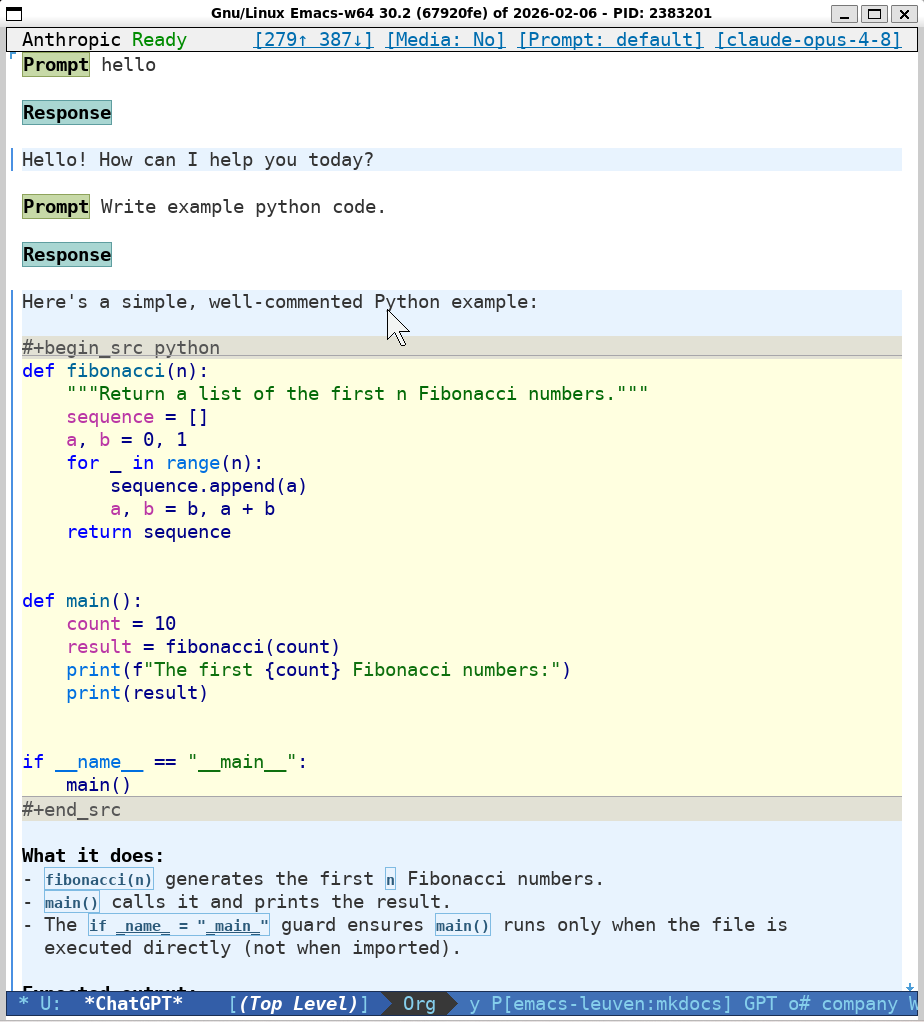
\includegraphics[width=.75\linewidth]{gptel-chat-buffer.png}
\end{center}

Référence :
\url{https://github.com/fniessen/emacs-leuven/blob/master/docs/emacs-leuven-gptel.txt\#17-chat-interface}
\subsection*{GPTel-commit-msg}
\label{sec:orgd298e03}

\textbf{But} : Générer des messages de commit Git à partir d'un buffer de diff avec
GPTel.

Le buffer de diff, quelle que soit la manière dont le diff a été produit (Magit,
VC, diff-mode, sortie de \verb|git diff|, etc.), est envoyé au backend GPTel configuré,
qui renvoie un message de commit décrivant les changements.

Le message obtenu est affiché dans un buffer séparé et copié dans le \emph{kill-ring}.

Référence :
\url{https://github.com/fniessen/gptel-commit-msg}
\section{Intégration avec le Shell}
\label{sec:orgb68f88c}

Quelques commandes permettent d'établir un pont pratique entre Emacs et le
terminal.

\begin{itemize}
\item \lstinline|e| pour ouvrir un fichier (ou un répertoire) dans l'instance Emacs en cours
à l'aide de \verb|emacsclient|~:

\begin{lstlisting}[language=shell,numbers=none]
  alias e='emacsclient -n -a emacs'
\end{lstlisting}

\item \lstinline|cate| pour afficher dans le terminal le contenu du buffer actuellement actif
dans Emacs.

\item \lstinline|cde| pour se placer dans le répertoire du fichier actuellement ouvert dans
Emacs.
\end{itemize}

Référence :
\url{https://github.com/fniessen/emacs-leuven/blob/master/docs/emacs-leuven.txt\#shell-utilities}
\section{Dotfiler (type Stow) pour tous mes repos}
\label{sec:orgc12dd3b}

\textbf{But} : gérer mes fichiers Org dans deux dépôts Git distincts (perso vs pro, ou
public vs privé), tout en y accédant depuis un seul répertoire logique unifié
sur la machine, via des \emph{symlinks}.

Les deux repos sont clonés séparément (ex. \verb|~/.dotfiles/org-perso| et
\verb|~/.dotfiles/org-pro|), et le dotfiler crée des liens symboliques vers un
répertoire unique, ex. \verb|~/org|.

Avantage : Un seul point d'entrée pour Emacs / Org-agenda; pas besoin de
multiplier les chemins dans la config.

Schéma simplifié :

\begin{verbatim}
[org-perso repo] ───┐
                    ├──symlinks──> [~/org/] <──── [Emacs/Org-agenda]
[org-pro repo]  ────┘
\end{verbatim}

\begin{itemize}
\item Les fichiers réels vivent dans le répertoire \verb|./org| de repos séparés
\item \verb|~/org| ne contient QUE des liens symboliques (\emph{symlinks})
\item Dotfiler crée/gère automatiquement ces liens
\item Emacs voit un seul dossier \verb|~/org| → simplicité de configuration
\item Chaque repo Git reste indépendant (historique, remote, accès séparés)
\end{itemize}

Le même principe s'applique pour \verb|bin/| et \verb|lisp/| : le vrai intérêt apparaît quand
on généralise ce mécanisme à \emph{tous} les répertoires \og fonctionnels\fg{} des repos, pas
seulement \verb|org/|.

Chaque repo peut avoir sa propre structure interne :

\begin{verbatim}
~/.dotfiles/repo-A/
├── org/     (fichiers Org)
├── bin/     (scripts perso)
└── lisp/    (paquets Elisp)

~/.dotfiles/repo-B/
├── org/
├── bin/
└── lisp/
\end{verbatim}

Dotfiler agrège alors chaque sous-dossier de chaque repo vers un répertoire
unifié correspondant :

\begin{verbatim}
repo-A/org/  ─┐
repo-B/org/  ─┴──symlinks──> ~/org/    <── Org-agenda

repo-A/bin/  ─┐
repo-B/bin/  ─┴──symlinks──> ~/bin/    <── $PATH

repo-A/lisp/ ─┐
repo-B/lisp/ ─┴──symlinks──> ~/lisp/   <── load-path Emacs
\end{verbatim}
\chapter{Formations EmacsBoost}
\label{sec:org70525c8}

L'objectif de mes formations est simple : transmettre toutes les fonctionnalités
d'Emacs que j'utilise au quotidien, et qui me font réellement gagner du temps.

Les formations mettent l'accent sur :

\begin{itemize}
\item les raccourcis utiles ;
\item Org mode ;
\item la gestion des projets ;
\item les automatisations ;
\item la personnalisation ;
\item les bonnes pratiques.
\end{itemize}

L'objectif est que les participants puissent appliquer immédiatement ce qu'ils
ont appris dès leur retour au travail.

Prochaine date à Paris : mars 2027.

Référence : \url{https://emacsboost.com}
\section{Témoignages}
\label{sec:org76b851a}

Quelques retours récurrents des participants :

\begin{itemize}
\item \og J'ai découvert énormément de fonctionnalités que je n'aurais jamais trouvées
seul.\fg{}
\item \og Le gain de productivité est immédiat.\fg{}
\item \og La formation est très concrète.\fg{}
\item \og Même après 20 ans d'utilisation quotidienne d'Emacs, j'ai appris énormément.\fg{}
\end{itemize}
\chapter{Merci}
\label{sec:org573e9e8}

Merci pour ton intérêt !

J'espère que cette conversation aura été une bonne occasion d'échanger quelques
idées, expériences et astuces autour d'Emacs, d'Org mode et de l'\emph{open source}.
\end{document}
